\section{Implementation}
\label{sec:md_implementation}
\subsection{Periodic boundary conditions}

\subsection{Two-body forces}
\label{sec:md_implementation_two_body_forces}
The Lennard-Jones potential gives rise to a two-body force acting only on pairs of atoms. In principle, this means we have to sum over all pairs in the system which for $n$ atoms in the system is $O(n^2)$. This calculation can be reduced to $O(n)$ by realizing that the gradient of the potential (hence the force) is nearly zero at $r \approx 2.5\sigma$, see figure \ref{fig:md_lennard_jones_2}. \todo{Show lennard jones force instead}
\begin{figure}[h]
\begin{center}
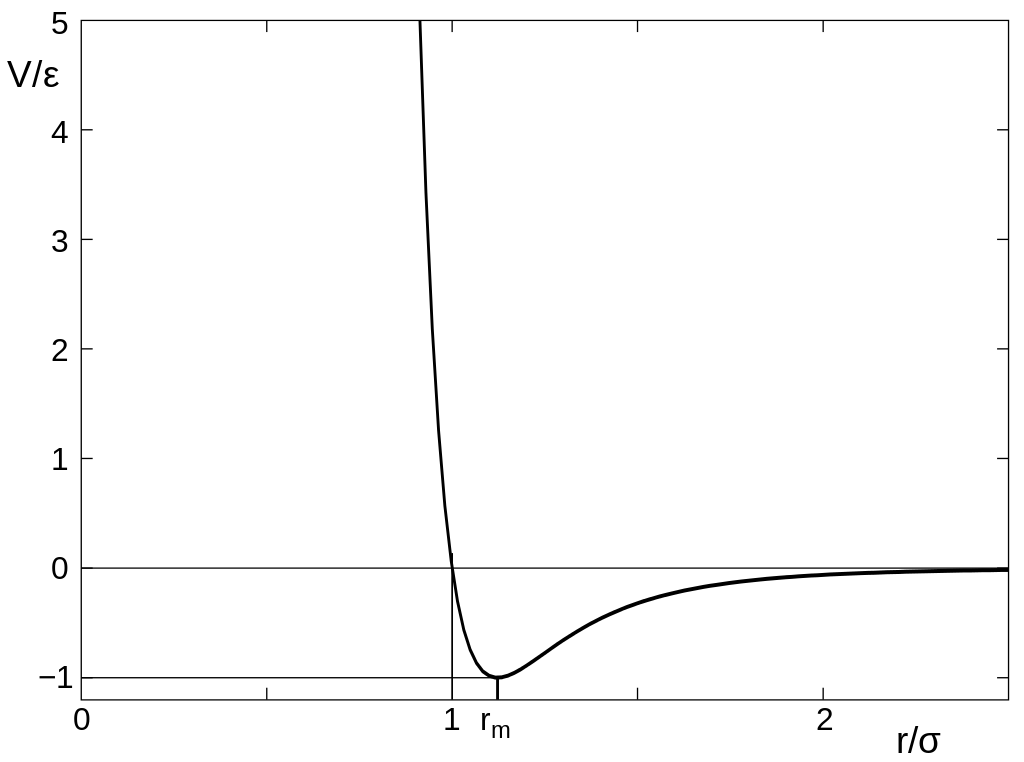
\includegraphics[width=1.0\textwidth, trim=0cm 0cm 0cm 0cm, clip]{MD/figures/lennard_jones.png}
\end{center}
\caption{The Lennard-Jones force. We see that the force is nearly zero at $r\approx 2.5\sigma$, so we don't need to calculate forces between atoms separated by a distance larger than $r_\text{cut} \equiv 2.5\sigma$.}
\label{fig:md_lennard_jones_2}
\end{figure}
We now introduce a certain cut-off distance $r_{cut}$ which we choose as the distance where the force is nearly zero, and set the force to be zero for any $r>r_{cut}$. The force between a pair of atoms $F(r_{ij})$ is then written as
\begin{align}
	F(r_{ij}) = \left\{\begin{array}{cc}
		F_{LJ}(r_{ij}) & \text{if } r \leq r_{cut}\\
		0 & \text{if } r > r_{cut}.
	\end{array}
	\right.
\end{align}
where $F_{LJ}$ is the standard Lennard-Jones force from eq \eqref{eq:md_lj_force}. We now don't need to sum over atom pairs of which the relative distance is larger than $r_cut$, so the calculation of forces is then globally $O(N)$. 